\section{Tri Thức Từ Vựng Học, Phân Đoạn Câu và Dóng Hàng Quy Hoạch Động Hai Tầng}

\subsection{Hợp nhất không gian từ điển đa nguồn và hệ âm đọc Nôm Công giáo}

Hiệu quả của các bước dóng hàng ngữ âm phụ thuộc trực tiếp vào độ phủ của ánh xạ giữa tự hình Hán Nôm và tập âm đọc hợp lệ $\mathcal{L}(c)$. Để giảm thiểu số trường hợp báo lệch do thiếu mục từ, hệ thống tổng hợp tri thức từ bảy nguồn từ điển ngữ văn và từ nguyên quy mô lớn, bao gồm \textit{Bảng chữ Hán Nôm chuẩn} ($8.855$ mục), \textit{Bảng Tra Chữ Nôm} ($13.443$ mục), \textit{Digitizing Vietnam} ($53.959$ mục), \textit{Đại Nam Quấc Âm Tự Vị} ấn bản năm $1895$ \cite{huinhtinh1895} ($70.364$ mục), \textit{Từ điển Hán Nôm HVDIC} ($50.332$ mục), cơ sở dữ liệu \textit{Unihan} \cite{unihan2025} ($132.698$ mục) cùng bảng quan hệ chữ dị thể \textit{CJKVI}. Sau khi chuẩn hóa về dạng dựng sẵn NFC, kho từ vựng hợp nhất đạt tổng cộng $329.651$ mục âm đọc, trong đó có $198.438$ mục âm Hán-Việt, Nôm và Quốc ngữ phủ trên $90.834$ tự hình đơn nhất, đi kèm $122.350$ liên kết dị thể hai chiều $V(c)$ giúp nhận diện các biến thể khắc chữ tương đương nhau về ngữ âm.

Mặc dù kho từ điển chung có độ phủ rộng, khảo sát trực tiếp trên hai tập sách cho thấy văn hiến Công giáo Việt Nam thế kỷ XVII--XX sử dụng một lớp từ vựng ký âm riêng lặp lại nhiều lần mà các từ điển thế tục không ghi nhận đầy đủ. Lớp từ vựng này gồm hai nhóm chính: nhóm danh từ riêng thần học đa âm tiết phiên âm từ tiếng Latinh hoặc Bồ Đào Nha như \nom{支秋} (\textit{Giê-su}, với \nom{秋} ghi âm \textit{su}), \nom{衣計移加} (\textit{I-ghe-rê-gia}, phiên âm từ \textit{Ecclesia} với \nom{計} đọc \textit{ghe} và \nom{移} đọc \textit{rê}), \nom{樞姚} (\textit{Giu-dêu}) hay \nom{樞蜂} (\textit{Giu-ong}); và nhóm chữ giả tá hay chuyển âm cổ trong ngữ cảnh giáo lý như \nom{最思} (\textit{tối tăm}, dùng \nom{思} đọc \textit{tăm}), \nom{諫讓} (\textit{khiêm nhường}, \nom{諫} đọc \textit{khiêm}), \nom{識傳} (\textit{Sấm Truyền}, \nom{識} đọc \textit{sấm}), \nom{偃㑏} (\textit{gìn giữ}, \nom{偃} đọc \textit{gìn}), \nom{𢗼憫} (\textit{lo lắng}, \nom{憫} đọc \textit{lắng}) và \nom{嚉靈魂} (\textit{rỗi linh hồn}, trong đó \nom{嚉} mang thêm âm \textit{rỗi} bên cạnh âm \textit{dối} thông thường). Việc bổ sung có chọn lọc lớp âm đọc chuyên biệt này vào không gian tra cứu giúp thuật toán dóng hàng phản ánh đúng tập quán ký âm của tác phẩm thay vì đánh dấu nhầm các thuật ngữ tôn giáo là lỗi nhận dạng.

\subsection{Khôi phục từ vắt dòng, nối câu xuyên trang và phân đoạn câu theo ngữ cảnh}

Trước khi thực hiện dóng hàng, các chuỗi văn bản rời rạc theo dòng và theo trang cần được tái cấu trúc thành những đơn vị câu hoàn chỉnh. Trên ấn bản Quốc ngữ đầu thế kỷ XX, trở ngại đầu tiên nằm ở dấu gạch nối cuối dòng vì nó vừa có thể là dấu nối nội tại của danh từ riêng phiên âm (như \textit{Giê-su}, \textit{Phi-ri-tô}), vừa có thể chỉ là ký hiệu ngắt dòng cơ học khi hết lề phải. Để phân giải sự nhập nhằng này, hệ thống xét đặc trưng viết hoa của hai mảnh $p_1\text{-}p_2$ qua điểm ngắt dòng: dạng nối liền $p_1\text{-}p_2$ được giữ lại khi cả hai mảnh đều viết hoa chữ cái đầu hoặc thuộc danh mục từ ghép cố định, còn các trường hợp từ thông thường được khôi phục thành hai âm tiết cách nhau bởi khoảng trắng.

Tiếp theo, do nhiều câu văn bắt đầu ở cuối trang $t$ và kéo dài sang đầu trang $t+1$, việc tách câu độc lập trên từng trang sẽ cắt đôi những câu vắt trang thành các mảnh thiếu đối ứng. Nhằm tránh hiện tượng này, hệ thống kiểm tra ký tự hữu ích cuối cùng trên vế Quốc ngữ của mỗi cặp trang (bỏ qua dấu đóng ngoặc hoặc dấu ngoặc kép đi kèm); nếu chưa xuất hiện dấu kết câu (\code{. ? ! ; : \ldots}), cặp trang hiện tại được gộp liên thông với cặp trang kế tiếp thành một cụm trang thống nhất trước khi phân đoạn, đồng thời lưu lại khoảng chỉ số ký tự của từng trang gốc để gán đúng định danh câu về trang chứa ký tự mở đầu. Trên chuỗi Quốc ngữ đã nối cụm trang, bộ phân đoạn ranh giới câu hoạt động theo hướng xét ngữ cảnh lấy cảm hứng từ mô hình Punkt \cite{kiss2006punkt}: thay vì tách cơ học tại mọi dấu chấm, thuật toán kiểm tra cặp từ liền kề $(w_i, w_{i+1})$ để không ngắt câu sau các chữ viết tắt đa chấm (\textit{v.v.}, \textit{đ.c.}) và viết tắt tôn giáo -- học thuật (\textit{Lm.}, \textit{Th.}, \textit{St.}, \textit{Đc.}, \textit{tr.}), không ngắt tại trích dẫn Kinh Thánh có ký hiệu sách (\textit{Mt, Mc, Lc, Ga, Rm, Cr, Tv,\ldots}) đi kèm số chương hoặc số câu, và không ngắt sau chữ số La Mã chỉ thứ tự mục khi từ kế tiếp $w_{i+1}$ bắt đầu bằng chữ cái viết thường hoặc không mang dấu hiệu mở câu mới.

\subsection{Quy hoạch động hai tầng}

Thách thức lớn nhất khi dóng hàng giữa văn bản Hán Nôm và bản phiên âm Quốc ngữ xuất phát từ sự chênh lệch về độ tin cậy của dấu ngắt câu ở hai hệ chữ viết. Trong khi bản Quốc ngữ có hệ thống dấu câu và quy tắc viết hoa đầu câu tương đối rõ ràng, bản Hán Nôm lại có nhiều đoạn kéo dài không chấm câu hoặc dùng dấu khuyên tròn \nom{。} lệch vị trí so với dấu chấm câu Quốc ngữ. Nếu tách câu độc lập trên cả hai vế rồi mới ghép cặp ở mức câu, chỉ một vài chỗ tách sai ở đầu trang cũng có thể kéo theo sai lệch cho các câu kế tiếp. Để khắc phục hạn chế này, quy trình dóng hàng được thiết kế theo mô hình \textbf{quy hoạch động phân cấp hai tầng} kết nối trực tiếp với kết quả từ bước hợp nhất ROVER như trình bày ở Hình~\ref{fig:rover_dp}.

\begin{figure}[H]
    \centering
    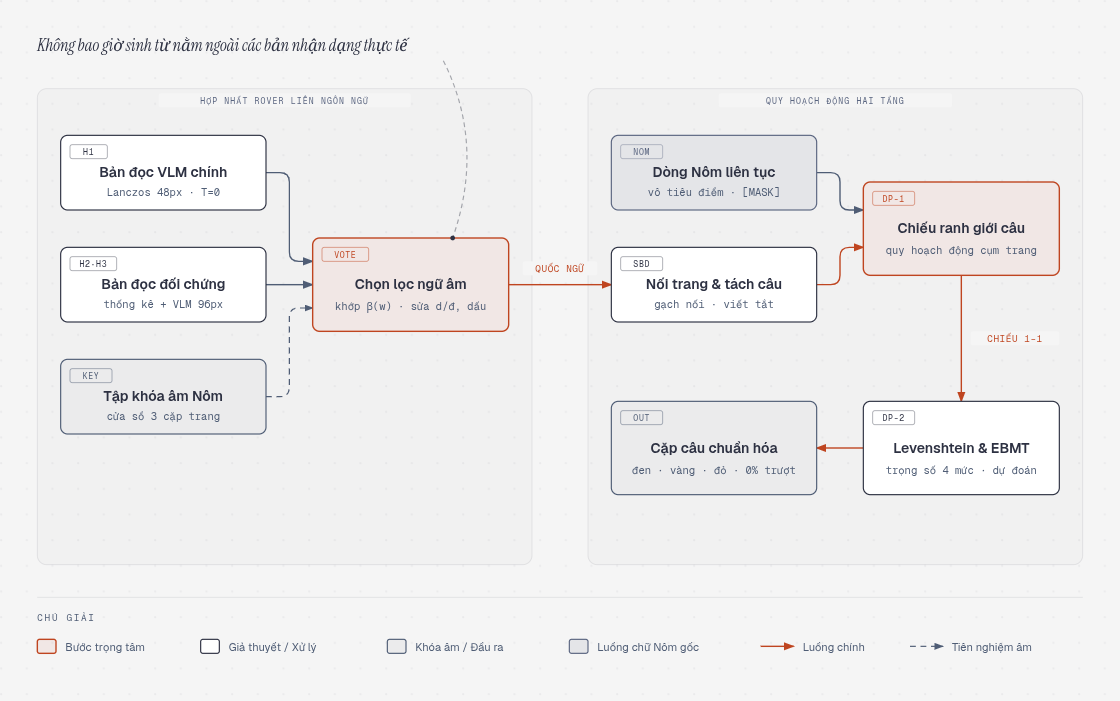
\includegraphics[width=0.95\linewidth]{images/fig2-rover-dp.png}
    \caption{Cơ chế hợp nhất ROVER liên ngôn ngữ kết nối với quy hoạch động phân cấp hai tầng}
    \label{fig:rover_dp}
\end{figure}

\subsubsection{Tầng 1: Chiếu ranh giới câu cấp độ cụm trang}

Trên mỗi cụm trang đã nối xuyên trang, gọi $C = (c_1, c_2, \dots, c_N)$ là dãy toàn bộ phần tử Hán Nôm (giữ nguyên dấu câu tại vị trí gốc và xem ký hiệu khuyết chữ \code{[MASK]} là một phần tử nguyên tử không chia tách) và gọi $S^{(1)}, S^{(2)}, \dots, S^{(K)}$ là $K$ câu Quốc ngữ đã tách theo ngữ cảnh, tạo thành dãy gồm $M$ âm tiết $S = (s_1, s_2, \dots, s_M)$ với các mốc ranh giới câu tích lũy $0 = \tau_0 < \tau_1 < \dots < \tau_K = M$. Thay vì tìm ranh giới câu trên vế Hán Nôm bằng dấu câu, tầng thứ nhất căn chỉnh trực tiếp chuỗi $C$ với chuỗi $S$ qua ma trận quy hoạch động $D \in \mathbb{R}^{(N+1) \times (M+1)}$ được xác định bởi điều kiện biên $D(0, 0) = 0$, $D(i, 0) = i$, $D(0, j) = j$ cùng hệ thức truy hồi:
\begin{equation}
    D(i, j) = \min
    \begin{cases}
        D(i-1, j-1) + \delta_{\text{lex}}(c_i, s_j) & \text{(khớp hoặc thay thế)} \\
        D(i-1, j) + 1 & \text{(xóa phần tử Nôm, bao gồm dấu câu Nôm)} \\
        D(i, j-1) + 1 & \text{(chèn âm tiết Quốc ngữ),}
    \end{cases}
\end{equation}
trong đó chi phí ngữ âm $\delta_{\text{lex}}(c_i, s_j)$ bằng $0$ nếu $s_j$ thuộc tập âm đọc trực tiếp $\mathcal{L}(c_i)$ hoặc tập âm đọc qua quan hệ dị thể $\bigcup_{v \in V(c_i)} \mathcal{L}(v)$, và bằng $1$ trong trường hợp còn lại.

Khi truy vết đường đi có tổng chi phí nhỏ nhất từ $(N, M)$ ngược về $(0, 0)$, các bước đi chéo xác định một ánh xạ đơn điệu không giảm $\mu: \operatorname{Dom}(\mu) \subseteq \{1,\dots,M\} \to \{1,\dots,N\}$. Với mỗi câu Quốc ngữ thứ $k$ nằm trên dải âm tiết $(\tau_{k-1}, \tau_k]$, chỉ số cắt kết thúc tương ứng trên dòng Hán Nôm $e_k$ được xác định tuần tự từ $e_0 = 0$ như sau:
\begin{equation}
    e_k =
    \begin{cases}
        N, & \text{nếu } k = K \\
        \max\Big(e_{k-1},\; \max\big\{\mu(j) \;\big|\; j \in (\tau_{k-1}, \tau_k] \cap \operatorname{Dom}(\mu)\big\}\Big), & \text{nếu tập ánh xạ khác rỗng} \\
        e_{k-1}, & \text{ngược lại.}
    \end{cases}
\end{equation}
Đoạn con liên tục $C[e_{k-1}+1 : e_k]$ chính là vế Hán Nôm tương ứng với câu Quốc ngữ thứ $k$, và mọi phân đoạn biên bị rỗng một vế (nếu phát sinh) sẽ được gộp vào câu liền kề. Nhờ cấu trúc phân hoạch nối tiếp này, tổng hợp tất cả các lát cắt câu luôn khớp từng ký tự với dòng Hán Nôm gốc trên cụm trang ($\bigoplus_{k=1}^K C^{(k)} \equiv C$), không làm rơi ký tự hay xé lẻ ký hiệu \code{[MASK]}. Quan trọng hơn, vì mỗi điểm cắt câu đều bám vào vị trí khớp ngữ âm thực trên toàn cụm trang thay vì dựa vào dấu \nom{。}, nhiễu cục bộ ở một câu không làm trượt ranh giới của những câu phía sau, giúp giữ tỷ lệ hàng không so sánh ở mức $0{,}00\%$ trên cả hai tập sách.

\subsubsection{Tầng 2: Đối chiếu chỉnh sửa Levenshtein có trọng số ngữ âm và phân lớp sai khác}

Sau khi có từng cặp câu 1--1 $(C^{(k)}, S^{(k)})$ ở dạng chuẩn hóa NFC, tầng thứ hai đối chiếu chi tiết từng tự hình Nôm với từng âm tiết Quốc ngữ. Trước hết, nếu hai vế có cùng số lượng ký hiệu khuyết chữ \code{[MASK]}, cặp câu được tách theo các điểm neo này để dóng hàng độc lập trên từng đoạn con, đảm bảo ký hiệu \code{[MASK]} luôn ở trạng thái trung lập và không bị tính là lỗi. Trên mỗi phân đoạn gồm dãy tự hình Nôm $(x_1, \dots, x_p)$ và dãy âm tiết hoặc số Quốc ngữ $(y_1, \dots, y_q)$, thuật toán khoảng cách chỉnh sửa Levenshtein \cite{levenshtein1966} sử dụng chi phí khoảng trống $w_{\text{gap}} = 1{,}0$ cùng hàm chi phí thay thế theo bốn mức ngữ nghĩa:
\begin{equation}
    w_{\text{sub}}(x_i, y_j) =
    \begin{cases}
        0{,}0 & \text{nếu } \phi(y_j) \in \mathcal{R}_0(x_i) \quad \text{(tương đồng âm đọc)} \\
        0{,}5 & \text{nếu } x_i \notin \operatorname{Dom}(\mathcal{R}_0) \text{ hoặc } y_j \text{ là chữ số} \quad \text{(ngoài từ điển hoặc số)} \\
        1{,}0 & \text{nếu } x_i = \text{``\nom{〓}''} \text{ hoặc } \big(x_i \in \operatorname{Dom}(\mathcal{R}_0) \land \phi(y_j) \notin \mathcal{R}_0(x_i)\big) \quad \text{(bất tương đồng).}
    \end{cases}
\end{equation}
Trong trường hợp xuất hiện nhiều đường truy vết đồng hạng chi phí, thuật toán ưu tiên phép chèn hoặc xóa trước phép thay thế nhằm gom gọn các ký tự bị nhận dạng lặp (chẳng hạn \nom{命命命} ứng với một âm \textit{Mình}) về phía cuối cụm.

Sau bước truy vết, các vị trí không khớp liền kề được gộp thành từng phần tử sai khác gắn tọa độ điểm mã nửa mở $[a, b)$ trên cả hai vế và quy về ba trạng thái trực quan. Những cặp khớp âm đọc trực tiếp cùng các ký hiệu \code{[MASK]} giữ trạng thái tương đồng (màu đen). Trạng thái cảnh báo hợp lệ (màu vàng) áp dụng cho các cụm chứa chữ số Ả Rập đối ứng với cách ghi số bằng chữ Nôm khác độ dài (ví dụ số \textit{1571} ứng với bảy chữ Nôm \textit{một nghìn năm trăm bảy mươi mốt}), danh từ riêng viết hoa có số chữ Nôm và số âm tiết không bằng nhau, cũng như các hàng có một vế được tổng hợp dự đoán do khuyết trang quét. Toàn bộ các sai lệch âm đọc thực sự, ký tự thừa hoặc thiếu, tự hình chưa có trong kho từ điển và ký tự đại diện ngoài chuẩn Unicode \nom{〓} đều được gán trạng thái bất tương đồng (màu đỏ) để phản ánh trung thực trong công thức tính điểm.

\subsection{Tổng hợp phiên âm dự đoán bằng dịch máy dựa trên ví dụ nội tại}

Đối với hai trang Hán Nôm ở Tập 1 bị thất lạc bản quét Quốc ngữ tương ứng (trang $358$ và $359$), việc tra thẳng từ điển tĩnh thường cho ra nhiều âm đọc khác nhau và dễ chọn nhầm âm không phù hợp với văn phong thế kỷ XX của cuốn sách; chẳng hạn chữ \nom{吧} trong từ điển phổ thông có âm \textit{ba}, nhưng xuyên suốt bộ sách này hầu như chỉ dùng để ghi liên từ \textit{và}, còn \nom{支秋} luôn được phiên thành \textit{Giê-su}. Để bám sát thói quen dịch âm của chính tác phẩm mà không cần tập huấn luyện bên ngoài, nhóm sử dụng phương pháp \textbf{dịch máy dựa trên ví dụ nội tại (In-Book Example-Based Machine Transliteration)}.

Cơ chế này gồm hai bước nối tiếp nhau trên cùng tập sách. Trước tiên, hệ thống duyệt qua toàn bộ các cặp câu đã dóng hàng của Tập 1 thỏa mãn điều kiện số lượng tự hình Hán Nôm bằng đúng số lượng âm tiết Quốc ngữ ($|X^{(r)}| = |Y^{(r)}| > 0$), rồi tích lũy bảng tần suất đồng xuất hiện $N_{\text{book}}(x_t, y_t)$ tại từng vị trí đối ứng $t$. Kế đến, với mỗi tự hình $c$ trên hai trang khuyết bản dịch, âm tiết dự đoán $\hat{y}(c)$ được chọn theo ước lượng hợp lý cực đại trên phân phối nội tại của cuốn sách và chỉ lùi về tra kho từ điển chung khi gặp tự hình chưa từng xuất hiện ở các cặp câu đẳng dài:
\begin{equation}
    \hat{y}(c) =
    \begin{cases}
        \arg\max_{y} N_{\text{book}}(c, y), & \text{nếu } \sum_{y} N_{\text{book}}(c, y) > 0 \\
        \min_{\text{lex}} \mathcal{L}(c), & \text{ngược lại.}
    \end{cases}
\end{equation}
Toàn bộ nội dung của hai hàng dự đoán này được đánh dấu cảnh báo màu vàng trên cả hai vế và giữ trạng thái chưa kiểm duyệt thủ công, nhờ đó tách bạch rõ khỏi mẫu số tính điểm tương đồng của phần văn bản có đủ ảnh gốc hai chiều.
